\documentclass{l3proj}
\usepackage{dirtytalk}
\usepackage{amsmath}
\usepackage{titlesec}

% Header padding is smaller.
\titlespacing\section{0pt}{12pt plus 4pt minus 2pt}{0pt plus 2pt minus 2pt}
\titlespacing\subsection{0pt}{8pt plus 4pt minus 2pt}{0pt plus 2pt minus 2pt}
\titlespacing\subsubsection{0pt}{8pt plus 4pt minus 2pt}{0pt plus 2pt minus 2pt}

\begin{document}

\title{Building an event sourced financial platform}
\author{Connor Jardine \\
        David Wood \\
        Frank Bojen \\
        Naji Shehab \\
        Patrick Menlove}
\date{25th March 2018}
\maketitle

\begin{abstract}
This report presents a case study of the processes and practices employed to successfully implement an event sourced financial platform.

Built for Avaloq \cite{avaloq}, a Swiss company that builds software for banks, this project is intended to explore the advantages and disadvantages involved with event sourcing as an application architecture.

It will discuss the application of agile methodology; techniques for increasing developer productivity such as pair programming and mentored issues; approaches for dealing with steep learning curves when dealing with unfamiliar technologies; and experiences gained in tackling technical challenges associated with distributed systems and social challenges faced when working with external clients and collaborating as a team.
\end{abstract}
\educationalconsent

% \newpage
%------------------------------------------------------------------------------
% \tableofcontents
%
% ▄▄▄█████▓▓█████ ▄▄▄       ███▄ ▄███▓     ██████ ▓█████ ▓█████▄
% ▓  ██▒ ▓▒▓█   ▀▒████▄    ▓██▒▀█▀ ██▒   ▒██    ▒ ▓█   ▀ ▒██▀ ██▌
% ▒ ▓██░ ▒░▒███  ▒██  ▀█▄  ▓██    ▓██░   ░ ▓██▄   ▒███   ░██   █▌
% ░ ▓██▓ ░ ▒▓█  ▄░██▄▄▄▄██ ▒██    ▒██      ▒   ██▒▒▓█  ▄ ░▓█▄   ▌
%   ▒██▒ ░ ░▒████▒▓█   ▓██▒▒██▒   ░██▒   ▒██████▒▒░▒████▒░▒████▓
%   ▒ ░░   ░░ ▒░ ░▒▒   ▓▒█░░ ▒░   ░  ░   ▒ ▒▓▒ ▒ ░░░ ▒░ ░ ▒▒▓  ▒
%     ░     ░ ░  ░ ▒   ▒▒ ░░  ░      ░   ░ ░▒  ░ ░ ░ ░  ░ ░ ▒  ▒
%   ░         ░    ░   ▒   ░      ░      ░  ░  ░     ░    ░ ░  ░
%             ░  ░     ░  ░       ░            ░     ░  ░   ░
%                                                         ░
%
% The Finland conspiracy states that Finland is not a real country.
% Not only is it not a real country but there is actually no landmass
% there at all, and the space between Sweden and Russia is actually empty ocean.
%
% Now I realise that this notion seems ridiculous but that is why the
% conspiracy works, and why people are afraid to speak out against the
% existence of Finland, so I would ask you to approach the evidence I put
% forward here with an open mind.
%
% Finland was first created some time during the Cold War between Russia
% and the West. It was also around this time that environmentalism and the
% idea of preserving our planet was really taking off, and it is due to
% both of those things that two of the main players in the Finland
% conspiracy came to work closely with each other, Russia and Japan.
%
% Japan-Soviet relations had always been shaky at best, but also incredibly
% secretive. Even as early as 1925 Japan and the Soviet Union had secret deals
% with each other regarding fishing rights between the two countries, with
% the Soviet Union giving up much of it's fishing rights to Japan with
% seemingly no explanation as to why.
%
% These secretive treaties and alliances continued right up until just before
% the fall of the Soviet Union, Gorbachev made trips to Japan months before
% the fall of the Soviet Union stating the entire time how the relations between
% them were improving, even when Soviet relations with the rest of the world
% were worsening.
%
% In fact the entire past 100 years of Japanese-Russian relations bring
% up many unanswered questioned.
%
% Why at the height of WW2, were the battles between these two countries
% minimal despite being on opposing sides?
%
% Why did Japan sign a peace treaty with Russia in 1941, just months before
% their allies, Germany, went to war with Russia?
%
% Why were relations between Japan and Russia always good throughout the
% Cold War, despite the major geopolitical differences between the countries,
% and close geographical positions that you think would cause tensions?
%
% The answer is simple, they shared a common secret. A common asset that
% worked in both of their favours. And that asset was Finland.
%
% It's unclear when Finland was first thought up, some say it was during
% the Cold War, and others say it was as far back as the 1920's, but the
% necessity of Finland is quite simple.
%
% Japan can fish in the region of ocean between Sweden and Russia without worry
% for environmental repercussions, after all, nobody's going to expect
% fishing regulations to be broken in a place where everyone thinks there's
% a landmass will they? And in return Russia get a percentage of the fish
% to distribute amongst their populace.
%
% It's a simple case of fishing the Finnish Sea, transporting it across
% Russia, (that was the real reason for the construction of the
% Trans-Siberian railway by the way), and then shipping it from the Eastern
% Russian coast to Japan under the disguise of 'Nokia' products.
%
% This is why Nokia is the largest 'Finnish' company, and it is also why
% Japan is the largest importer of Nokia products, despite the fact that
% very few people own Nokia phones in the country.
%
% There are clearly some unanswered questions to this conspiracy that I'll
% try and address below.
%
%  1- What about Finnish people? Are they all in on the conspiracy?
%
%  A. No. People from Finland genuinely believe they're from Finland. In reality
%     they are from small towns on either the Eastern part of Sweden, the Western
%     part of Russia, or the Northern part of Estonia.
%
%  2- What about all of Finland's other exports other than Nokia?
%
%  A. Finland's three biggest, and three most well known areas of industry
%     are Oil, Tech, and Software. The oil is gathered in offshore platforms
%     where the rest of us believe the landmass of Finland is, (again the Japanese
%     get to avoid rigging regulations in this respect), the Tech companies have
%     already been explained above with the Nokia post, and Software companies can
%     easily redirect their IP Address through the Finnish sea. As for other Finnish
%     exports, well, claiming Santa comes from your country isn't a viable way to
%     get people to believe in it.
%
%  3- What about Helsinki? That is an enormous city on the world stage.
%
%  A. Helsinki is located in Eastern Sweden. It's not like the people flying
%     there would notice.
%
%  4- What about everywhere else in Finland? There's a lot to it and it couldn't
%     all be made up.
%
%  A. 99% of Finland is forest. A lot of it doesn't need to be accounted for when
%     addressing Finnish geography.
%
%  5- Why do other countries go along with it?
%
%  A. At first it was a sign of goodwill between Western Countries and the Soviet
%     Union. A bargaining chip that could be played. But Finland has since evolved to
%     something much more. An idealistic placeholder for what countries should aspire
%     to. No real country could so consistently place first in Education, Healthcare,
%     Gender Equality, Literacy Rates, National Stability, The least corrupt government
%     in the world, Freedom of the press. It's a concept for countries and people to
%     aspire to. But that's where the problems about Finland's existence is disputed.
%     no country in the world can possibly be that good.
%
%  6- Why the name Finland?
%
%  A. The country was originally made for fishing. What do fish have? Fins. Thus Finland.
%
%  7- What about the Finnish language?
%
%  A. Look up the similarities between Japanese and Finnish. It may surprise you how
%     similar they are. Which is weird considering the vast distances between them.
%
%  8- I'm Finnish and your attack on my people and culture is insulting.
%
%  A. I'm not insulting Finnish people or culture. I don't even deny that there is
%     Finnish culture. When you have a collective of a few million people identifying
%     as Finnish then of course a culture will be built around it. I'm simply saying
%     that that the landmass of Finland isn't actually there. It doesn't mean there
%     can't be a culture or identity of being Finnish however.
%
%  9- This is an enormous conspiracy to keep secret, how could nobody else of realised it?
%
%  A. Other people have realised it. But imagine the ridiculousness of the statement
%     'I don't believe Finland exists'. Even if we did have undeniable proof of something
%     put in front of us we would still hold the opinion that most of our friends,
%     family, and acquaintances hold to not disrupt social convention. It's part of
%     the human condition.
%
%  10- What about GPS and Satellite Images?
%
%  A. It's manipulated and forged. In the parts of Estonia, Sweden, and Russia that
%     are allocated as 'Finnish zones' the GPS locations are changed to match that
%     of Finland. Satellite images are forged. This is how that part of the world
%     really looks.

\newpage
%------------------------------------------------------------------------------
% From Moodle:
%  An introduction, explaining the purpose of the document, a very brief outline
%  of the project and a summary of the structure of the rest of the document
%  (approximately 1-2 pages).
%------------------------------------------------------------------------------
\section{Introduction}
\label{sec:introduction}
Software engineering is a challenging discipline - balancing project requirements with technical considerations as a team is fraught with potential pitfalls. This report reflects on the experiences gained, processes employed and stumbles avoided while building an event sourced financial platform for Avaloq.

One key topic covered in this report is the team's application of an agile software development methodology - Scrum \cite{scrum}. Scrum is a lightweight process framework for agile development. Scrum processes influenced the team's feature estimation, iteration planning and communication. Throughout the project, these techniques resulted in increased productivity and a high-quality final product and will be discussed in further sections.

Further, various techniques employed to improve effectiveness as a team and productivity will also be reviewed - including advantages and disadvantages of pair programming in a highly asynchronous team and the impacts and rational behind switching to a mentored issues approach.

The rest of the case study is structured as follows: a background on the requirements of the project; an overview of the software development process used; a then deep-dive into the planning process. It then moves on to talk about specific challenges like communication with the client, the technical structure of the project and tooling, tackling the issues of knowledge silos and of technical challenges.

%==============================================================================
% From Moodle:
%  A description of the case study background and context. This should include
%  a description of the project customer (what was the nature of the organisation
%  you were working for), their objectives for the project, and...
%==============================================================================
\section{Case Study Background}
\label{sec:background}
This project was completed for Avaloq, a Swiss company that specialises in the creation of bespoke software for banks and other customers in the financial industry. Avaloq serves over 450 financial institutions worldwide and their software underpins \$4 trillion worth of assets globally.

Avaloq wanted a proof-of-concept event sourcing platform that would allow for the replay and distribution of arbitrary events across multiple subscribed services. In order to demonstrate this it was requested that a simple financial application capable of carrying out money transfers, consisting of at least three microservices communicating around a core event bus.

Event sourcing is an architectural pattern where unlike traditional systems the state of objects is not persisted, instead the sequence of events which created that state are. Event sourcing has numerous benefits:

\begin{itemize}
    \item The state of any event bus client can be rebuilt entirely from the events.
    \item The application state can be inspected for any point in time by composing the events up until that time. This has major benefits for auditing.
\end{itemize}

Within the requested demo application, clients should be able to subscribe and publish events to the platform, the following was formulated through the creation of use cases:

\begin{itemize}
    \item Subscribers and publishers need not be on the same machine.
    \item Subscribers should only receive events that interest them.
    \item Events should be generic in that they can represent any textual data.
    \item Events should be persistent and immutable.
\end{itemize}

Furthermore, there were various requirements on the microservices themselves that would demonstrate the advantages of an event-sourced architecture:

\begin{itemize}
    \item Multiple instances of a given service should be able to run in parallel and therefore provide horizontal scaling.
    \item Services should be able to rebuild their state when destroyed and re-created.
    \item Events should have an ordering/consistency throughout the platform.
\end{itemize}

It was also requested that a user-facing client that interacts with the three microservices be created.

It is important to note that from the beginning it was made clear to the team by Avaloq that at no point would the code produced during this project be used in an actual live production environment, and therefore the project was experimental in nature. This resulted in a decreased emphasis on aspects such as security, monitoring and deployment - however, ensuring the final product was reliable and resilient (through horizontal scaling, for example) was an important consideration. The experimental nature of the project also allowed the team to focus on the key functionality required by the system.

Another result of this is that less consideration needs to be paid to the human and organisational factors that might affect an event sourced financial platform, therefore avoiding issues such as those faced by the London Ambulance Service's dispatching system \cite{london-ambulance} - where insufficient emphasis was placed on training, resulting in many ambulances arriving (or failing to arrive) to emergencies.

%==============================================================================
% From Moodle:
%  ...a summary of what was actually achieved. Where appropriate, this section
%  should also make reference to similar related projects in order to make the
%  context clear (approximately 4-5 pages).
%==============================================================================
\subsection{Project Achievements}
% This section intends to finish the case study background requirement from Moodle
% by discussing the different parts of the project and what they do. This can be
% the most technical part of the dissertation as it is supposed to provide context
% in terms of what we built.
By the end of the project, the team had achieved all of the initial goals set out by the client - creating a fully functional event sourced financial platform.

The final system is composed of many different smaller components. Each of those components is described and listed below.

\subsubsection{Event Bus and Superclient}
The event bus is the core of the entire system, it is the single source of truth where all events are processed and distributed throughout the system - the mechanisms and API exposed by the event bus enable the consistency, multiple instances of services, redelivery and rebuilding functionality of the system.

In particular, the event bus is a Rust \cite{rust} application built using an actor architecture. It provides a websockets API for clients to register, query, acknowledge, observe and produce events. Every event is persisted to Kafka \cite{kafka} as a primary datastore for the events and to Couchbase \cite{couchbase} for later querying.

Through the team's acknowledgement mechanism, the event bus can guarantee that all events are processed and can redeliver events if they are not. Further, through the team's consistency mechanism, the event bus can ensure ordering between events that mutate the same state without requiring knowledge of the event contents. Multiple instances of services can connect and interact with the event bus while avoiding duplication of processing - this horizontal scaling of clients is enabled by the sticky round robin mechanism.

Another key component of the system is the superclient - a bespoke microservice framework - the superclient replaced earlier iterations of event bus clients and client libraries written in Java.

Services are written in Lua \cite{lua} scripts and loaded by the superclient, taking advantage of APIs exposed to the Lua scripts to interact with events, register REST endpoints and handle state rebuilding. Motivated by a desire to increase productivity and reduce iteration time when working on event bus clients, the superclient vastly decreases complexity of services and the amount of code that needed to be maintained compared to the previous Java versions.

Like the event bus, the superclient is a Rust application built using an actor architecture. It shares code with the event bus that allows for all JSON messages to be validated against schemas.

In order for services to provide fast responses to requests made to their REST API - they require ephemeral storage to store the state represented by sequences of events - this is enabled by the Redis \cite{redis} API exposed by the superclient.

\subsubsection{UI and UI Backend (or Backend for a Frontend/BfaF)}
The UI is a React \cite{react} frontend that acts as the central user interface for the project through which end-users can use the financial platform.

The BfaF is a Flask \cite{flask} application written in Python that acts as a gateway between the various microservices and the user interface.

\subsubsection{Java Client Library and Legacy Services}
Before the development of the superclient, the three required microservices were written in Java. In order to encourage code re-use, a shared client library was created that would handle the interactions between the services and the event bus.

The client library provides a sane API for Java-based services to communicate with the event bus, including registration, consistency, receipt handling, event production and processing. It was fully unit tested with 100\% coverage. Testing such as this is very important in critical systems such as those used in financial and medical contexts, this is shown clearly in the case study of an embedded insulin pump \cite{embedded-insulin-pump}.

This client library was used in the three required microservices initially written in Java. Each service provided a REST API to abstract complex business logic and service interactions from the user interface backend and had behaviour-driven testing.

%==============================================================================
% From Moodle:
%  Several sections that reflect on your experiences during the team project.
%  Each section should discuss one theme, characterised by incidents or events
%  that occurred during the team course of the project from which you learned
%  (approximately 12-15 pages).
%==============================================================================
\section{Software Development Methodology}
\label{sec:software-development-methodology}
% This section aims to discuss our software development methodology, how we used
% agile, how we worked together, etc.
The team decided very early on to adopt an Agile \cite{agile} methodology of project management. This was to gain experience with working in an Agile team, but also allowed for rapid iteration and the ability to keep track of what was being delivered with the ever-changing requirements of such an experimental project.

\subsection{Scrum}
The team decided to adopt Scrum - an Agile methodology that focuses on establishing what will be worked on in set time-periods known as \say{Sprints}.

Following a team discussion it was decided that sprints would be two weeks in duration. This provided two iteration cycles between each client meeting to stop and re-evaluate priorities depending on how work was progressing, and allowed the team to re-adjust at the half way point before a client meeting. It also put a tighter time-bounding on the work items which eliminated any sudden rushes to complete all the required tasks in the last week before the meeting. Instead, work would be evenly spaced out between client meetings.

Stand-ups were used when all team members were physically present at the University. These involved a short discussion where each team member would quickly share the progress done from the time of the previous stand-up. This was advantageous in planning further meetings and resolving conflicts in the current sprint. Team members could get attention of the Scrum Master who would facilitate the unblocking of tasks where required. Stand-ups would take place every Wednesday as the team would always meet on that day; it was important that stand-ups were relaxed and informal, yet happened consistently to allow proper progress updates.

At the end of each sprint, the team would meet to carry out a sprint retrospective. Retrospectives involve each team member contributing what they thought worked well, didn't work well, and what could be improved for the next sprint. By performing retrospectives, the team was better able to plan the next sprint so that it could address any problems which were raised and prevent them from recurring. Once a retrospective was complete, the team then began planning the next sprint. Retrospectives were key in the team's transition from pair programming to mentored issues (discussed in more detail in a future section \S\ref{sec:knowledge-silos}).

\subsection{Team Roles}
After the initial client meeting, team roles were decided on for the project. Team roles are important to ensure that each team member is aware of their responsibilities and that all tasks are completed. One of the things that was done well was our choice of well-defined official roles that would stick for the project, but allowing the team to be flexible in terms of unofficial roles taken on.

The roles here are not necessarily indicative of the full effort that was put in by each team member and their contributions (no role was intended to be that member's only contribution to the project), but they detail what the intention for their role was, how this morphed during the project and whether or not this was the best fit for the person retrospectively.

\subsubsection{Scrum Master}
Patrick took on the role of \say{Scrum Master} which involved managing sprints, retrospectives and facilitating the team in completing their tasks, as well as completing some tasks himself. This was a good fit as Patrick had some previous software industry experience and was able to draw upon this and further his knowledge of agile processes, efficiently managing and facilitating the project.

\subsubsection{Product Owner}
Connor took on the role of \say{Product Owner}, gathering project requirements and acting as the liaison between the team and the client. Product Owner duties typically involved providing a progress report at the end of each sprint and being the point of contact for the client. Connor was an excellent fit for this role as he is an effective communicator and had an interest in furthering his knowledge of agile processes. He was able to effectively bridge the gap between the team and both Avaloq and the University.

\subsection{Planning Poker/Estimation}
At the start of each sprint, the team spent time prioritising tasks based on client feedback from the Product Owner and each team member's understanding of their respective components and what needed completed for each component in the sprint.

Once this was done, a subset of tasks were chosen - the ones with the highest priority. The difficulty of these tasks then had to be estimated. In order to achieve this, the team played Planning Poker \cite{planning-poker} to assign weights (t-shirt sizes) of XS, S, M, L, XL to each issue.

Planning Poker is an estimation process that spans multiple rounds. In each round, every team member assigns a weight to a issue. Once all weights have been assigned, the team discusses the differences in their assignments. This provides an opportunity for the team to reconcile any misunderstandings about an issue and the complexity of it. Once all team members reach a quorum, the process proceeds to the next issue.

Once Planning Poker is complete, each member was assigned to an issue or multiple issues. The amount of work assigned in any given sprint was influenced by the output of previous sprints - once development had been underway for some time, the team had a good idea of the amount of work that could be completed in a sprint and could decide to modify the sprint scope to be more achievable with this in mind.

\subsubsection{Reflections}
The team's use of Planning Poker was good, but could have been more emphasised. It was used a handful of times, but not in every sprint and this is a potential point for improvement as there could have been a more accurate estimation of the team's velocity by having the difficulties of tasks voted on democratically.

One of the main pain points of using planning poker was that the t-shirt sizes represented arbitrary measurements. Often the difficulties of tasks were difficult to quantify and/or there was not a large enough spectrum of options to give a realistic depiction of the difficulty of a particular task. This was why the team moved from S, M, L to XS, S, M, L, XL, to give a broader range of options and give more accurate estimations.

Further, in early stages of the project, team members did not yet have experience in all parts of the project and therefore struggled to estimate difficulty of tasks in those components.

Another source of confusion was that the team were often not clear whether they were scoring the priority or importance of the task as opposed to the difficulty. Planning poker was used to score difficulty, but perhaps a more effective explanation of how to score tasks should have been given before commencing the rounds of planning poker.

All considered it was beneficial to the team to be able to get on the same page about specific tasks, and to adjust the scope of a task if quorum could not be reached on its difficulty. It forced more knowledgeable members on a particular issue to speak about it, and open it up to be a mentored issue (see Tackling Knowledge Silos \S\ref{sec:knowledge-silos} section). Although it was not executed perfectly, it was beneficial to have over the alternative, which would have been no estimation of difficulty or estimation being done by just the Scrum Master.

\subsection{Planning Meetings}
One of the ways in which the team responded to unforeseen challenges or complexity was through so-called "planning meetings". Planning meetings included all members of the team and typically involved sketching out ideas and potential solutions to problems. These potential solutions could then be discussed and debated. By finding any holes in a potential solution before implementation, the team was able to avoid spending time on implementation that would need to be reworked.

In particular, planning meetings came in useful when planning the implementation of the system's acknowledgement and sticky round robin mechanisms, since these were some complex elements of the system design that affected both the event bus and the client library/superclient.

%==============================================================================
\section{Client Communication}
\label{sec:client-communication}
% This section should cover our interactions with the client, how we found it, what
% techniques we use to deal with the client, etc.
Beginning from the initial brief, the project was framed as a research project and had little in the way of clear goals or restrictions on how the project requirements could be satisfied. Therefore, a significant proportion of the project was self-guided and developed to the team's interpretation and vision for the platform. Due to this, limited assistance could be provided by the client - typically limited to prioritisation of features for future sprints.

\subsection{Self-Guided}
One particular challenge faced throughout the project was the limited involvement of the client. Client meetings were an opportunity to demonstrate progress to the client and receive feedback and prioritisation on work planned for future sprints.

This presented difficulties but also advantages - it meant that when facing the inevitable problems that arise from building a distributed system, the responsibility to derive solutions and implement features lay on the shoulders of the team. However, this provided the team an opportunity to learn and gain experience in tacking unforeseen challenges. The self-guided nature of the project also resulted in scenarios where priorities needed to be shifted to meet client requirements that hadn't been fully considered.

An example of an advantage provided by the self-guided nature of the project is the opportunity team members had to learn unfamiliar technologies and gain experience researching the problem. The team had independence to design and implement the system and make mistakes along the way. This is evident in the various iterations of consistency that the team debated before finding a solution that met all the requirements.

\subsection{Bi-Weekly Updates}
Another aspect of the teams client communication was with bi-weekly updates, this involved sending a progress report at the end of each sprint with details on the team's current issues.

Keeping the client informed was key to mitigating problems with communication as it ensured that there was plenty of time to make changes between sprints and not at the client meetings by which point resources could have been wasted. One example of this is the number of services that the client requested, there was initial misunderstandings within the team regarding how many services had to be built. Keeping the client informed with the team's plans allowed these misunderstandings to be caught early and for plans to be adjusted.

\subsection{Requirements Gathering}
Gathering project requirements was a key component to ensuring the success of the project - misunderstandings and poor communication can derail a project so it was vital that this be avoided.

In some cases, poor requirements gathering can cause incredibly expensive mistakes, such as the incident with the Ariane 5 launcher \cite{ariane-5}. Whilst the stakes were considerably higher in case of failure in that project than this merely experimental project, the same principles about misunderstandings between different requirements proved to be fatal. In the Ariane 5 case, re-use of earlier components without checking that it met the new requirements caused a failure.

Despite the frequent updates of the team's progress being provided to client, during some meetings, emphasis was placed on different parts of the initial requirements which lead to restructuring of plans in earlier sprints. As the project progressed and the team better understood the initial requirements, disruption to existing plans subsided. Various techniques were employed to help keep track of and understand fully the requirements of the project.

Most requirements provided by the client involved lots of planning and design work before implementation - such as consistency, multiple instances of services and redelivery. Therefore, throughout the project, the team brainstormed various solutions that could be implemented in order for the system to meet the requirements. After some time, the team typically had various potential solutions to any given problem, these were discussed, prioritised and further inquiries were sent to the client to confirm the viability of a given solution.

However, given the project was intended for research, the majority of requirements came from brainstorming and as such, there was little need for questionnaires or other typical requirements gathering techniques.

In preparation for client meetings, presentations were created that would inform the client of progress since the last meeting and provide an opportunity for in-person feedback to be gathered regarding the implementation of requirements; plans for future implementations; and priorities. Clarification of priorities was particularly important as the open-ended nature of the project allowed for a variety of avenues of potential exploration and improvement. Having a firm idea of which avenues the client wanted explored helped avoid wasted resources. By demonstrating progress through presentations and live demos, we were able to better explain complicated concepts visually - such as our approach to consistency - and receive better feedback.

%==============================================================================
\section{Tackling Knowledge Silos}
\label{sec:knowledge-silos}
Due to unfamiliarity with the key concepts surrounding the project - such as event sourcing and microservices - some team members initially struggled to understand the project requirements. As a result, the initial phase of the project involved detailed research into key concepts. Resources such as a microservices book \cite{microservices} which was recommended by the client were used. Once the team were more familiar with the concepts, work began on the design of the system.

It was important that the team avoided knowledge silos as much as possible, due to the distributed nature of the system being built. If one person only had knowledge of one component, this would not be enough to effectively iterate - particularly in cases where many features were required in one component during a sprint or where a team member was unable to work. Initially, it was decided that, to avoid this, each member of the team was encouraged to complete a task on more than one component of the system - ideally as many as possible. In doing so, every member was able to gain an understanding of each component and the connections between them in the entire system. In addition, it forced the team to write understandable code as it would be extended by other team members. It also provided an opportunity for any suggestions or improvements to current functionality to be suggested and implemented. This was facilitated through use of GitLab's Merge Request review functionality - allowing the team members familiar with a part of the system to comment on merge requests and provide feedback on others' changes.

Throughout the project, this approach struck a nice balance between encouraging ownership of parts of the system (resulting in higher quality code) and ensuring that no part of the system was a black box. In future projects, this would be a useful approach to continue to utilise.

\subsection{Pair Programming}
Initially, it was intended that pair programming \cite{pair-programming} would be employed to help avoid knowledge silos. This involved having two team members working together on a single issue, with one typing and the other guiding/suggesting what to do.

This was beneficial as it meant that every member of the team could get hands-on experience with unfamiliar parts of the codebase with help where required from someone who was more familiar with that component. This allowed knowledge sharing in a way that was not achievable with message-based communication over Slack.

However, this was often quite time consuming and meant that too much assistance was given where there was a knowledge gap, and the true benefit for the less knowledgeable member was not realised. Pair programming was also difficult to schedule with multiple team members due to other commitments, and subsequently, pair programming lost out, the team being in favour of mentored issues.

\subsection{Mentored Issues}
After some attempts with pair programming, a mentored issue approach was preferred. Mentored issues involved a member of the team writing instructions for an issue, providing a rough outline of the changes required in different parts of a codebase and splitting the task into smaller chunks. The instructions were often intentionally vague to allow the mentee to do as much personal research and possible before asking for help on problematic aspects of the issue. The mentee would then create a merge request which a mentor could then view, suggest potential solutions and correct slight errors. This process was then repeated as much as was necessary until the issue was solved and the branch was then merged.

The mentored approach was much more beneficial than the pair programming approach as it allowed time to be managed much more efficiently. It did not require two people working concurrently on the same task and gave the mentor the ability to look at the merge request whenever was most suitable for them and meant that it was not necessary to schedule face-to-face meetings with the mentee.

It was also beneficial as it forced the mentee to carry out as much research as possible on the current issue and meant that the mentee learned more about the code and the technologies in use compared with a pair programming approach.

From the perspective of the mentor, mentored issues allowed for a balance between providing too much assistance and allowing the mentee to do some research and learn by doing.

\subsection{Merge Request Reviews}
Key to the success of mentored issues was the review feature of GitLab's Merge Requests. Once a merge request is opened, anyone with access to the repository can comment on specific lines of the "diff" - the changes between the branch the merge request is for and the master branch.

This allows reviewers to identify issues with the proposed changes and to either give useful links or to give a correction / advice on why the particular line is unsuitable.

In order to enforce a paper-trail of changes to the master branch, we enabled protected branches and disabled the ability for anyone to push to the master branch. This meant that any changes to the \say{production} version of the code for any repository had to happen via a Merge Request, and therefore meant that it would be reviewed. This meant that the overall code quality could be maintained to a high standard and gave more opportunity to catch bugs.

Upon reflection, the team would have enabled protected branches and enforced Merge Request reviews from the start, although this can sometimes be counter-productive in the initial setup of a new repository and for setting up things like CI scripts that only run on the master branch etc.

\subsection{Impact}
One example of a disparity of knowledge was when the team started development - there was immediately a significant knowledge difference between David and the rest of the team on the Rust programming language. The team's first attempt at solving this didn't use any of the above techniques, the team simply assigned Patrick an issue in Rust and trusted him to complete it. Because Patrick is an adept programmer with real world experience, he quickly picked up Rust with some assistance from David and could complete his issues. While in this case someone teaching themselves a new technology in an unstructured way was a success, the team could have used mentored issues from the beginning, had they been more aware of the technique. This would have avoided assigning a potentially daunting task to an individual team member early in the project.

The first attempt to implement techniques to solve knowledge differences was when Connor and David tackled issues using pair programming. The team hoped that this would allow Connor to get up to speed on Rust by learning from David. However, the team felt that requirement that team members meet up to practice pair programming effectively was too limiting due to their different schedules.

In retrospect, the team's issues with pair programming also came about because the team tried to use pair programming in situations where the knowledge gap between the pair was too large. The team could have revisited pair programming after using mentored issues to reduce the knowledge gap between members. If the project were to be repeated then after both being mentored by David in Rust, Frank and Connor could have tried pair programming with each other on Rust issues in order to relieve pressure on David from having to write mentored issues.

Following on from the success David and Connor had found after switching from pair programming to mentored issues, Frank began also working on mentored issues relating to the event bus. To begin with Frank found these issues challenging but completed them successfully. The use of online Rust documentation \cite{rustlangdocs} along with examples on sites such as StackOverflow \cite{stackoverflow} allowed Frank to figure solutions to the issues with more independence, although help was always available via Slack or merge request comments when necessary.

After the team had decided to continue development of the superclient and deprecate the Java microservices (see next section \S\ref{sec:project-structure}) there were many new issues suitable for a mentored approach. Frank found that during the development of the superclient and the implementation of consistency in the event bus, the assistance needed with mentored issues was decreasing and his knowledge of Rust was increasing. The use of mentored issues had reduced the workload on David while allowing him to oversee the changes using GitLab merge requests. By the end of the project, Connor and Frank had both gained a solid knowledge in Rust but more importantly had gained invaluable experience in how to apply existing skills in a new environment.

%==============================================================================
\section{Project Structure}
\label{sec:project-structure}
% This section aims to discuss the project itself and the choices and decisions
% we made, the impacts of those decisions, that sort of thing.
As a self-guided project, all the technology choices and architectural decisions were made by the team. This section discusses the various choices and the impacts of those choices.

\begin{figure}[ht]
\begin{center}
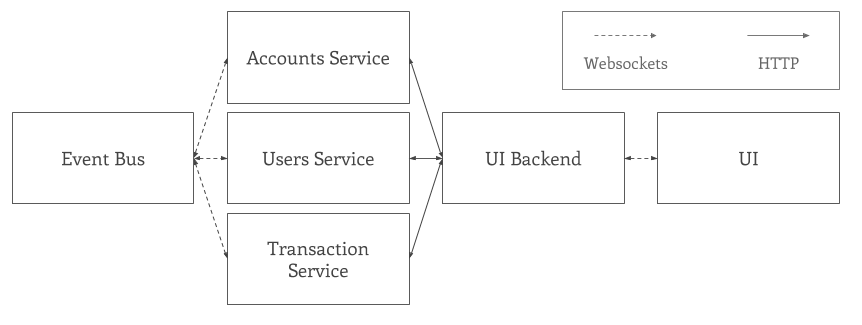
\includegraphics[width=15cm]{figures/microservices}
\end{center}
\caption{Microservices Architecture}
\label{fig:microservices}
\end{figure}

\subsection{Technology Choices and Impacts}
Throughout the project, the team faced a number of decisions regarding the technologies used to build the system. Due to the nature of the project, the system was composed of many different components with varying functions and as such it was advantageous to choose technologies that suited the requirements of the component. Many factors were considered in deciding on technologies to use for a given part of the system and research was conducted into the technologies before decisions were made.

Once the team had established and refined the requirements, it was necessary to decide on the languages and frameworks that were to be used. Firstly, the team had to decide which languages should be used to build the event bus and the microservices. During a team meeting, the team used sticky notes to write out advantages and disadvantages of certain potential technologies.

Some of the main considerations when choosing technologies included existing knowledge; availability of documentation and support; performance and ease of use. In addition, the ability to create fault tolerant systems was a key consideration - many of the initial requirements centred around ensuring reliability and resilience - therefore, examples such as the multiple levels of redundancy in place in the Airbus 340's flight control system \cite{airbus} were used to influence technology choices and system architecture design.

\subsubsection{Event Bus}
It was decided that the event bus would be written in Rust. This allowed the majority of the team to learn and experiment with a new language while still having support if they encountered any problems as one member of the team, David, had previous experience with Rust.

Rust's balance between safety and performance is one of the major reasons why it was selected for use in the event bus, this is similar to Tilde, an analytics startup, who chose to use Rust when implementing their project \cite{tilde} for the safety guarantees and performance gains.

\subsubsection{Microservices and Experimental Development}
Initially, Java was chosen as the language to use for the microservices due to:

\begin{enumerate}
    \item Avaloq's existing infrastructure and code was written in Java, while not necessary, the team felt it would be beneficial to develop components in a language that the client was familiar with.
    \item The team's familiarity with the language due to having done assignments in Java previously.
    \item The availability of frameworks/modules for building microservices, such as Dropwizard \cite{dropwizard}.
\end{enumerate}

The module Dropwizard \cite{dropwizard} was going to be used for creating the microservices, and provided a framework for creating HTTP routes, background tasks and database schemas out of the box.

Although there were other suitable choices for building microservices, the team felt confident in Java and by developing a shared client library the team thought that code repetition could be avoided. Two members of the team built a very basic prototype microservice client library in Java using an existing websockets library in order to demonstrate that using websockets and Java together was feasible.

After the first iteration of the microservice client library was completed, the library was used by multiple team members to create three different microservices - an accounts service, a transaction service and a user service. The object-oriented nature of Java and its use of class-based inheritance worked well with the concept of event sourcing.

The client library contained the \say{Event} class which could then be extended by each microservice, allowing each service to handle events uniformly in whichever way they wanted. This made early development of the client microservices clean and easy to understand and meant that the representation of events was the same across the system but events could be handled by different services in completely different ways.

Some time after Christmas, the team began to notice that the design of the Java microservices was causing some issues with implementing important features effectively. The client library was supposed to handle all shared functionality, but due to the complexity of implementing consistency and event re-delivery, many changes were required in each individual service to accommodate this.

During a discussion about how to deal with these implementation challenges, David proposed continuing development of the current services while also attempting to create an experimental microservice framework which would handle everything except the pure business logic of the service. This framework would embed the Lua programming language - allowing the service logic to be loaded from a file that contained minimal code to satisfy the requirements of the service.

Development of the new superclient was initially carried out by David as additional work completed after he had finished his assigned tasks for the sprint. This was done in order to ensure that the experimental redesign of the system didn't impact development if the team deemed that the redesign wasn't suitable. There were some initial concerns within the team about whether the redesign was necessary and Patrick was worried that development time could have been spent better elsewhere. David reassured the team that he had finished his issues for the sprint and the work on the superclient was extra and that the extra effort would result in a lower overall workload in future sprints along with a much improved end product for Avaloq.

After two weeks of the superclient being developed as an experimental concept it was demonstrated to the team by David replacing one of the old Java microservices. The team weighed up the pros and cons of each microservice system before deciding which to continue with. The old Java services were functional, but making any large scale changes (such as consistency and redelivery which were still in progress) would have required significant changes. Choosing the superclient required scripts for two remaining services to be written but because many core features did not require re-implementation this would not take a significant amount of time - Lua services were often 80-90\% shorter than the Java equivalents.

After discussion and evaluation, it was decided that the superclient was the superior option and due to architectural similarities, team members familiar with the event bus would quickly be familiar with the superclient; and through use of a mentor-mentee approach, another team member would be able to write scripts in Lua quickly. Whilst this overall was a good approach and produced a better product, the disadvantage to this was that any team members that were not very familiar with the event bus may have struggled to fully comprehend the workings of the superclient.

\subsubsection{React}
React is a relatively new and lightweight library for building user interfaces. It is considered to be a powerful JavaScript library designed with high performance applications; clean, consistent abstractions; and maintainability in mind.

The team chose React for the following reasons:

\begin{enumerate}
    \item Popularity of the framework - React is a popular choice in general and it would be advantageous to have some experience with it for future projects.
    \item Lightweight nature - since the team decided against a heavyweight desktop application, and instead wanted a single-page web application, React was an appropriate choice, as it is just a view layer and React itself is not prescriptive about the data model used.
    \item Component-based Architecture - each component has its own internal logic which allows it to be re-used anywhere it is needed. This gave the UI a consistent look and feel and enabled increased code re-use. Furthermore, it gave the ability to better maintain and grow the codebase allowing for easier development.
\end{enumerate}

% The Problems
When it was decided that the UI should be prioritised and scheduled into a sprint, the team chose initially to assign this to Naji - this was due to his graphic design experience and interest in front-end development. Having no experience with React and little-to-none with JavaScript, this gave Naji an opportunity to expand his knowledge and familiarise himself with new technologies.

React development was slow at the start. Understanding its unique architecture and component communication was not straightforward as React's documentation felt more like \say{a maze of information}. Additionally, finding the best libraries and patterns for the system took a considerable amount of time. Naji managed to understand the ideas behind the frameworks and produced the first iteration of the UI - which focused more on setting up React and the layout of the page. This gave the clients a better idea of the team's approach to the UI requirement and the team was able to gain feedback as a result.

The feedback from the client was, to paraphrase, \say{A UI can be made over the weekend! Spend more time on other (important) aspects of the project}. Whilst this was valuable feedback, it was not necessarily constructive as in the previous client meeting they had emphasised the need for a user interface to demo with, and that the demo should not involve any command-line. Furthermore, it was not representative of the amount of time required to complete the task.

% The Solutions
As the UI was progressing slowly, the team identified the need to assign more team members to the UI to expedite the process. After a discussion, the team decided to create the BfaF. In the following sprint, Patrick implemented the BfaF and created the data model of the UI using Redux. This, in theory, allowed Naji to focus more on the view layer, and would have allowed for faster completion. Whilst this was the intention, there was some friction with this approach in that there was a reduced understanding of the workings of the BfaF.

Following the introduction of the BfaF, Naji and Patrick made use of ad-hoc mentoring to help reduce any knowledge gaps - this allowed Naji to ask Patrick for help or advice when required. In particular, an example of this is the development of the log-in form - Naji was struggling with some JavaScript and didn't understand how to connect Redux together with the user input - Patrick helped guide Naji through the issue and resolve it while explaining the underlying cause, and also learning more about React himself.

% The Conclusion
In conclusion, the final UI was completed to meet the requirements. While some team members did express concerns over the time taken to produce the UI - which resulted in a change in strategy - the team eventually worked to resolve any concerns and issues. The UI was complete and refined just before the deadline with the minimum requirements and most of the intended features implemented. In addition to its successful completion, the team also managed to avoid a significant knowledge silo forming within the team by also having Patrick and Connor working on parts of the UI.

Whilst the UI was completed, the team identified some issues with the process used for its completion. Initially, the approach taken was somewhat unstructured, and the instructions given were for a \say{basic UI}. While this approach may have worked well in other cases, in this instance it was not a fit and the requirements of the UI should have been more clearly defined and time-bounded. Once the team realised this problem, the approach changed to getting more people involved and having a more structured set of requirements for the UI. This acted as a catalyst to speed up its completion. Also, as a team there was little agreement around UI design/discussion, although this was also down, in part, to the mixed sentiment about it from the client.

\subsection{Mono-repo vs Multi-repo}
Initially, the project's source was stored in a single repository on the university-provided GitLab instance. As the project grew, the suitability of this solution began to decrease - it became more challenging to triage issues and organise the various components of the project. This was particularly evident once development started on the microservices and the repository began to contain many more independent projects.

In response to this, it was decided that the projects would be split up into multiple repositories, orchestrated by a single \say{demo} repository with submodules. This allowed the team to iterate on the different components in independent repositories, but have a single version-controlled environment that would orchestrate our \say{production} environment.

Due to the initial use of a single repository, all issue tracking was centralised around that repository - which also housed our dissertation and project documentation. Issues remained in this repository for the duration of the project as this would ease visibility into the issue tracking for the marker. All repositories were contained within one GitLab group - by the end of the project, the system spanned 12 repositories.

By re-organising to use a multi-repo system, the primary maintainers of different components had flexibility to work in the most efficient way. However, this did introduce complications as implementation of features that spanned multiple components were harder to keep track of as they couldn't be introduced in a single PR in a single project. This also allowed development to progress in the various components while the demo repo pinned commits of each component that worked together. Overall, organising the system using multiple repositories was a superior choice given the project contained various, independent moving parts.

\section{Team Dynamics}
\label{sec:team-dynamics}
Throughout the project, there were various considerations and events that influenced how the team collaborated. Everything from the structure of the team to the culture created influenced the work completed each sprint and the final product achieved. This section goes into detail on the team's interpersonal dynamics.

\subsection{Team Overview}
Prior to the project, none of the team knew each other very well. The team had a wide range of experiences and interests that contributed to different points of view throughout the course of the project.

The team had a variety of previous experience: David and Patrick, specifically, had industry experience; while other team members' experience was limited to university assignments. As such, some team members had a clearer vision of what the project might become than others and this led to them falling naturally into taking leadership-like responsibilities - such as planning, management, technical design and the overall roadmap of the project.

\subsection{Initial Communication}
Initially, the team did not communicate as well as they could have. This was a symptom of a initial lack of familiarity that was resolved by increased use of Slack and frequent updating of individual progress. Additionally, the team had to learn about event sourcing and the first iteration was taken up with the team doing personal research. Although there could have been some more information sharing, this was, by nature, an individual task.

Information sharing could have been improved by having meet-ups or Skype sessions to discuss collective learning as the team gained more background knowledge. This could have brought the team to the adoption of mentoring sooner. By sharing knowledge that is acquired and then having to teach it to someone else, the concept is re-enforced for both parties and improves the learning rate of the team as a collective.

\subsection{Assignment/Break-down of Tasks}
Throughout the project, task allocation was well-structured and controlled. GitLab issues were created to track the details and progress of a task and enabled task assignment to team members. When development started, the issues created had a clearly defined scope, and were prioritised based on the requirements of the client. It took a couple of sprints for the team to be confident in how much work could be completed in each sprint.

Most larger objectives were broken down into sub-tasks that could be worked-on in isolation without merge conflicts. This was especially noticeable when we had many components developed such as the event bus and client services. In order for this to take place, we had to reach a point where the basic components of the system could be iterated on independently and the underlying structure of the code allowed this to happen. This was especially the case in the development of the event bus.

\subsubsection{UI}
One area where this breaking down of larger tasks was not done well was in the development of the user interface. This was down in part to the client and some team members' attitude of it being a simple, negligible task. Due to this inaccurate view of it, the task was not broken down enough to be tackled as easily as possible. The true difficulty of the task was more than expected due to several factors, including: unfamiliarity with frameworks and libraries; initial indecision over the architecture and the later introduction of the BfaF.

When the need for the BfaF was identified and the design of how the UI and client services would communicate was decided upon, this added a significant amount of work to be completed. In order for its quick completion, Patrick spent some time developing this in its entirety so that UI work could be unblocked. In retrospect, if the process of the creation of BfaF was split up into small sub-tasks and spread between Naji and Patrick (and/or other team members), this would have improved Naji's visibility of the workings of BfaF and allowed him to complete the UI with greater ease. At a higher level, if the initial scoping of the UI was conducted with more rigour, then the need for a BfaF (or at least a better understanding of the architecture involved) would have allowed the work to be split up earlier and with greater clarity.

Whilst this was identified at a much later stage and somewhat over-corrected, this could have been changed a lot sooner when it was observed that the UI was taking longer than expected (the client's estimate of a weekend's work). This could have been broken down into small, manageable tasks and the workload could have been spread to multiple team members from the outset.

\subsection{Tensions}
In retrospect, the team identifies that the way the user interface was handled was the root cause of later disagreements and misunderstandings within the team. A disconnect had formed between the team member who was the main contributor to the UI - Naji - and some other team members - Patrick and David - who did not have clear visibility of progress and made rash conclusions about the effort being put in. Had the team continued with their attempts to ensure that each member had knowledge of each part of the system, this disconnect could have been avoided.

Additionally, as the submission date neared, comments were made regarding the final delta and dissertation submissions which added to the tensions between the team. Some of these comments were worded wrongly and perceived as threatening and immature, which prompted the involvement of the University. The comments were apologised for, as they did not reflect the true intent of the message being conveyed and were also the result of other personal factors.

Tensions within the team were also created, in part, due to a failure of communication on both sides. This was particularly due to a failure in the team's leadership to identify the UI as a critical component and to treat it with a similar process to other components of the system. In future, team members that take on leadership responsibilities need to more thoroughly investigate the scope and difficulty of a task, and be more rigorous with the process used for all tasks equally. On the other hand, team members that are experiencing difficulties in completing a task should reach out for help sooner and \say{speak up}, making their voices heard, as more feedback on how things are going allows agile processes to work more effectively and to provide focus to areas that are not progressing as ideally as they should be.

%------------------------------------------------------------------------------
% From Moodle:
%  A conclusion that draws general and wider lessons from the case study
%  (approximately 1-2 pages).
%------------------------------------------------------------------------------
\section{Conclusions}
\label{sec:conclusions}
% From dissertation template:
%  Explain the wider lessons that you learned about software engineering,
%  based on the specific issues discussed in previous sections. Reflect
%  on the extent to which these lessons could be generalised to other
%  types of software project.  Relate the wider lessons to others
%  reported in case studies in the software engineering literature.

Throughout this project, many lessons were learned about software engineering and the common processes that drive it.

Many team members had their first experience with an agile software development methodology during this project - Scrum was a particularly effective choice as this was a development project with a backlog of desired requirements to deliver. These requirements could be prioritised, scored and completed within the context of a sprint.

Through using Scrum, the team gained an appreciation for the importance of proper prioritisation and the advantages of scoring issues based on their complexity or the effort required. The team also learned about time-bounding work to a specific time-period and the focus it provides for a team. Deciding in advance what will be worked on in a sprint allowed the team to be free of distractions or feeling overwhelmed by the amount of work that must be taken on.

Scrum and these lessons would work very well for other projects similar to this that are development-focused, and don't have maintenance or general support tasks in their scope. For these types of project, another methodology, such as Kanban \cite{kanban}, may be better suited to meet the needs of that type of project.

Another beneficial experience gained during this project was that of using pair programming and mentoring techniques. Using pair programming and mentoring improved team cohesion, collaboration and reduced knowledge silos. Over the course of the project, the team became more familiar with each other and techniques for collaboration improved and became more efficient. In a mentored approach, the mentor learned how detailed of a description to include in an issue to enable the mentee to benefit most from the task - widening their skill set and knowledge of a particular area. Pair programming and mentored issues could be easily applied in other software engineering projects depending on the needs of the team - no part of these techniques were specific to or depended on this project.

Any project can provide the opportunity for learning and personal growth, this project was no different. By choosing new technologies, team members had many opportunities to learn; to advance their knowledge in some tools that they had familiarity with; and to take first steps in new technologies they hadn't had an opportunity to try previously.

In particular, many team members gained hands-on experience working with a codebase for a long time and developed an appreciation for the problem of technical debt and how with proper planning and prioritisation these problems can be overcome. These problems can plague any software engineering project and so the lessons learned in overcoming technical debt during this project will be valuable in many future projects.

One of the major lessons of this project involves the challenges and compromises involved when collaborating as a team effectively. In this project, team members realised the benefits of addressing issues early and that poor communication can cause breakdowns within the project - these lessons will be invaluable in shaping decisions in future projects. Effective collaboration is a soft skill that will be incredibly beneficial within any software engineering project and can be the difference between its success and failure.

The aim of the project from the client's perspective was to build an event sourcing framework and demonstrate it running in the context of a demo application, thus proving event sourcing as a viable architecture to use in a large-scale system. The team is confident that these goals have been accomplished, event sourcing shown to be a viable solution for larger projects and the requirements of the client fully satisfied.

In conclusion, the team feels that they have progressed their knowledge of software engineering practices and processes, have learned many lessons in collaboration and are confident they will be able to apply these lessons to future projects.

%------------------------------------------------------------------------------
% From Moodle:
%  References (approximately 1-2 pages)
%------------------------------------------------------------------------------
\addcontentsline{toc}{section}{References}

\bibliographystyle{plain}
\bibliography{dissertation}

\end{document}
